\documentclass{report}
\usepackage[utf8]{inputenc}

% Títulos automáticos en español
\usepackage[english]{babel}

% Soporte para buenas urls e hipervínculos entre secciones
\usepackage{hyperref}

% Citas y referencias en formato APA
% Si quiere las citas y referencias en IEEE comente esta línea
\usepackage{apacite}

% Imágenes y figuras
\usepackage{graphicx}

% Código fuente con números de línea
\usepackage{listings}
% Puede cambiar el lenguaje de código fuente
% https://www.overleaf.com/learn/latex/code_listing#Supported_languages
\lstset{
    language=C,
    basicstyle=\footnotesize,
    numbers=left,
    stepnumber=1,
    showstringspaces=false,
    tabsize=1,
    breaklines=true,
    breakatwhitespace=false,
}


\def \unidad{University of Milan}
\def \programa{Master in Data Science and Economics}
\def \curso{Fintech Industry}
\def \titulo{Kickstarter }
\def \subtitulo {Fintech project}
\def \autores{
    Andrea Ierardi\\
   Student ID: 960188
    \vspace{0.5cm}
    
  
}
\def \fecha{March 2021}
\def \lugar{
    Milan
}


\makeatletter
\def\@makechapterhead#1{%
  \vspace*{50\p@}%
  {\parindent \z@ \raggedright \normalfont
    \ifnum \c@secnumdepth >\m@ne
      \if@mainmatter
        %\huge\bfseries \@chapapp\space \thechapter
        \Huge\bfseries \thechapter.\space%
        %\par\nobreak
        %\vskip 20\p@
      \fi
    \fi
    \interlinepenalty\@M
    \Huge \bfseries #1\par\nobreak
    \vskip 40\p@
  }}
\makeatother

% Inicia el documento 
\begin{document}

% Inserta la portada del documento
\begin{titlepage}
    \begin{center}
        \vspace*{1cm}
        
        
\includegraphics[width=0.8\linewidth]{figuras/logo_tec.jpg}\\
        \LARGE
        \unidad\\
        \programa\\
        \curso
        
        \vspace{1cm}
        
        \Huge
        \textbf{\titulo}
            
        \vspace{0.5cm}
        \LARGE
        \subtitulo
            
        \vspace{1.5cm}
        
        \large    
        \autores
            
        \vfill
        
        \lugar\\
        \fecha
        
    \end{center}
\end{titlepage}

\tableofcontents

\chapter{Introduction}\label{intro}
\begin{figure}
    \centering
    
\includegraphics[width=0.6\linewidth]{figuras/kickstarter_logo.png}
    \caption{Kickstarter's logo}
    \label{fig:ksl}
\end{figure}
Kickstarter (Figure \ref{fig:ksl}) is an American public benefit corporation based in Brooklyn, New York, that maintains a global crowdfunding platform focused on creativity. The company's stated mission is to "help bring creative projects to life". The platform, launched in 2009, has developed almost 200.000 businesses and projects collectively raise \$5.6 billion in funding. Over all the 500.000 project, the 38\% of them have been successful.  


\section{How it works}\label{antecedentes}
Kickstarter is specifically for creative projects in the following categories: Art, Comics, Crafts, Dance, Design, Fashion, Film/Video, Food, Games, Journalism, Music, Photography, Publishing, Technology, and Theater. Many small businesses can fit into this categories. It is a marketplace where people with creative ideas meet people who want to support these ideas and buy innovative products. The creators launch their project on the platform with a set funding goal. They explain the idea using images, videos and rewards to backers. The rewards can be divided in tiers based on the amount of the support they receive from the backers. Once the funding goal is achieved, the backers' cards are charged with the amount they've pledged and the amount is transferred to the creators. The backers, then, will receive the rewards as promised.  

\newpage
\section{Kickstarter Terminology}\label{terminology}
Kickstarter uses a specific terminology:
\begin{itemize}
    \item \textbf{Creators}: individuals or groups who request funding for a project (with a clear goal). They start a Kickstarter Campaign, requesting funding. 
    \item \textbf{Backers} : people who pledge money for the funding of creators' projects. They are the ones that creators need to appeal to. They may support a product voluntarily or looking for returns out of them. Returns can be free products, offers, discounts, event invites etc.
    \item \textbf{Project}: the idea brought to life by creators. It is a work with a clear goal around which Kickstarter's business model revolves. The project can be visualised in the web-page on Kickstarter platform that lays out all the detail of a project.
    \item \textbf{Funding goal}: the amount of money needed to complete the project. All the projects start with a predetermined funding goal. The creator receive money only after the project reaches the funding goals. Also, backers' cards are charged only when project is fully funded.
    \item \textbf{Rewards}: The experiences or product that backers receive from the creator in exchange for their financial support. It could be an experience, limited editions, copies of their creative work, video call with the creator or also giving name to some character of an artwork. 
\end{itemize}
\section{Start a campaign}\label{campaign}
Starting a project is simple: 
\begin{enumerate}
    \item \textbf{Create an account}: it takes just few minutes, inserting some personal information and the password. Also, there are three steps in which it is needed to write the project's name and category. 
    \item \textbf{Describe your project} (Figure \ref{fig:prj}): this is the most important step for a creator. It is the key to whether the project will be successful or not. Kickstarter also provides a Creator Book in which are described some tips on how to effectively starts a project. In fact the main part of starting a campaign is finding a suitable idea but also find a suitable amount of fund to ask to the Backers. Moreover, in the book it is suggested to includes video, picture for a better story telling.  
    \item \textbf{Set your rewards}: it is needed to set up a credible goal and suitable rewards to give to the backers in exchange to their financial support. 
    \item \textbf{Connect you bank account}: the last step is connecting business bank account to the Kickstarter account so that it is possible to receive the funds.
    
\end{enumerate}

\begin{figure}
    \centering
    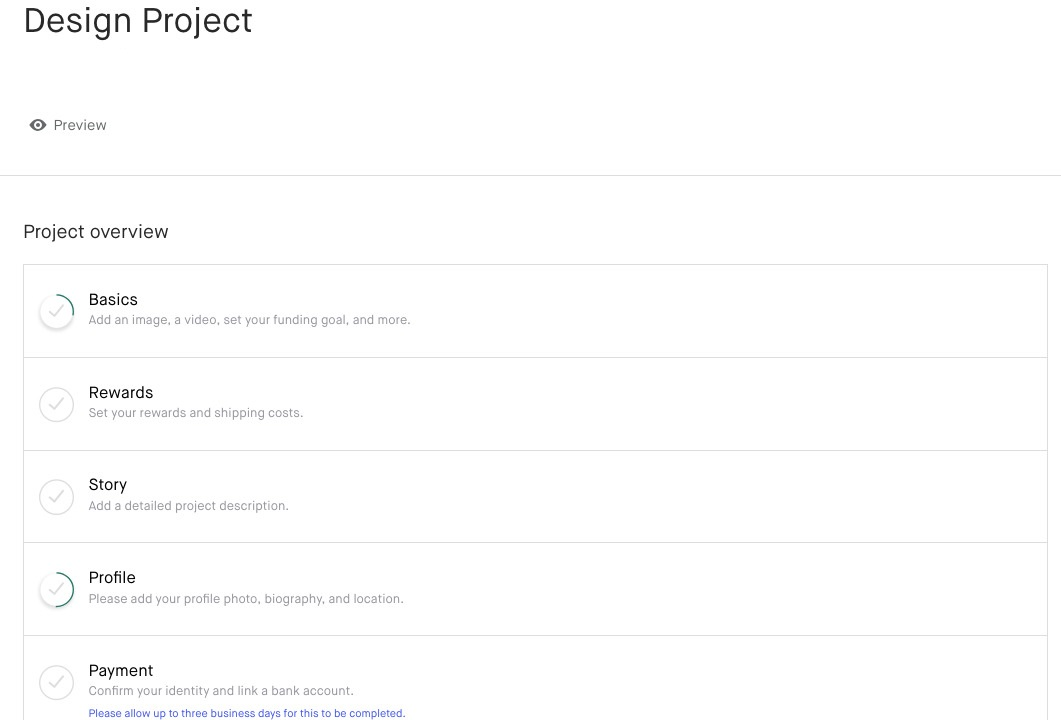
\includegraphics[width=0.85\linewidth]{figuras/project.jpg}
    \caption{Project designing}
    \label{fig:prj}
\end{figure}

\section{Limitations}
Kickstarter is open to backers all over the world. Anyone, from anywhere, can pledge to a project as long as they have a major debit or credit card.
Project creation is currently available to individuals who meet the below requirements in the following countries: US, UK, Canada, Australia, New Zealand, the Netherlands, Denmark, Ireland, Norway, Sweden, Germany, France, Spain, Italy, Austria, Belgium, Switzerland, Luxembourg, Hong Kong, Singapore, Mexico, Japan, Poland, Greece, and Slovenia.
Moreover, there are other \textbf{constrains}:
\begin{itemize}
\item You must be 18 years of age or older. People under the age of 18 can launch projects only in collaboration with an adult.
\item You must be a permanent resident of one of the above listed eligible countries
\item You must create a project in your own name, or on behalf of a registered legal entity with which you are affiliated
\item You must have an address, bank account, and government-issued ID based in the country that you're creating a project in
\item If running your project as an individual, the linked bank account must belong to the person who verified their identity for your project
\item You must have a major credit or debit card
\item You must have the authority to represent the organization to our payments partner
\end{itemize}

\chapter{Business model}\label{businessmodel}
\section{Customer Segments}\label{customerseg}
Kickstarter has a multi-sided business model, with two interdependent customer segments that are both needed in order to operate: creators and backers. Two-sided networks can be found in many industries, sharing the space with traditional product and service offerings. Example markets include credit cards (composed of cardholders and merchants); health maintenance organizations (patients and doctors); operating systems (end-users and developers); yellow pages (advertisers and consumers); video-game consoles (gamers and game developers); recruitment sites (job seekers and recruiters); search engines (advertisers and users); and communication networks, such as the Internet.

\section{Value Proposition}\label{valueprop}
It offers a set of primary value propositions: accessibility, risk reduction, performance and brand.
\begin{enumerate}
    \item \textbf{Accessibility}: the project is available online on a web-page but also in mobile applications;
    \item \textbf{Risk reduction}: the start-up does not have to put any investment and money to start a campaign. If the project does not get full funding, they could move to another idea. If they get full funding, they have the money to complete the project;
    \item \textbf{Performance}: the platform manage all the backers automatically;
    \item \textbf{Brand}: it gives the possibility to the start-up to create a community supporting the project.
\end{enumerate}

\newpage
\section{Key activities}\label{keysact}
Kickstarter's business model entails maintaining an active platform between creators and backers. The company main resource is its technology employees who maintain the platform. 
The company does not have dedicated partner program, but has partnered with various entities for cross-promotional purposes.

\section{Cost Structure} \label{costs}
It has a cost-driven structure and the objective of minimizing expenses through automation. The biggest costs are likely in the areas of customer support and administration, which are both fixed costs.

\section{Earnings} \label{earnings}
It is a for profit business even though is a crowdfunding company. The company earns its revenue by charging a 5\% commission fee on the total funds raised. They also charge a separate fee for payment processing which is between 3\% and 5\%. Pledges under \$10 have a discounted total fee of 5\% + \$0.05 per pledge, which is a way of encouraging creators to raise small amounts of money from a large number of backers.

\section{Example of the most funded project}
The Pebble Time (Figure \ref{fig:peb}) is the largest successful Kickstarter campaign.
Pebble Time is a smartwatch developed by Pebble Technology and assembled by Foxlink, released on 14 May 2015. This is the first Pebble to introduce a color e-paper display, as well as a microphone, a new charging cable and a new Pebble Time-optimized operating system.
In early 2015, Pebble announced the product, as well as its fundraising on Kickstarter. The watch received \$1M in 49 minutes, breaking a current record, and became the most funded Kickstarter to date, reaching \$20.4M all the way to its deadline, from over 78,741 backers.
\begin{figure}
    \centering
    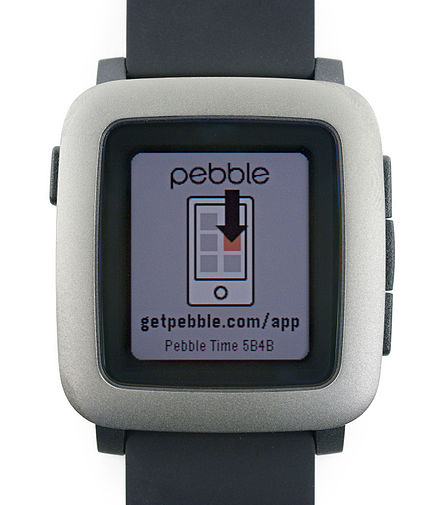
\includegraphics[width=0.2\linewidth]{figuras/pebble.jpg}
    \caption{Pebble product}
    \label{fig:peb}
\end{figure}

\chapter{Conclusion}\label{conclusion}
Kickstarter's mission is to help bring creative projects to life. They believe that art and creative expression are essential to a healthy and vibrant society, and the space to create requires protection. Also they does not want art world elites and entertainment executives to define our culture; they want creative people to take the wheel and they help creators connect directly with their communities, putting power where it belongs.
Kickstarter is growing day by day as the number of projects launched in the platform. It is important not only in spreading ideas, but also in creating a community around these ideas. The platform started in 2009 and projects collectively raise \$5.6 billion now. 
\\\\
Citing De La Soul, an American hip hop group that get his project funded: \textit{“Kickstarter is one of those platforms that gives you space to work with people who know you, love you, and support you.”}

\newpage

\chapter{Reference} \label{reference}
\begin{itemize}
\item \url{https://www.inc.com/guides/2010/04/using-kickstarter-for-business.html}
\item \url{https://www.investopedia.com/ask/answers/120214/how-does-kickstarter-make-money.asp}
\item \url{https://www.fundera.com/blog/kickstarter-for-business}
\item \url{https://www.cleverism.com/company/kickstarter/}
\item \url{https://www.feedough.com/payment-gateway-business-model-how-payment-gateways-work/}    
\item \url{https://www.kickstarter.com/help/stats?ref=hello}  
\item \url{https://www.investopedia.com/terms/b/businessmodel.asp}  
\item \url{https://articles.bplans.com/how-to-launch-an-awesome-kickstarter-campaign}  
\end{itemize}
 
% Estilo de bibliografía APA
% Si quiere usar el estilo IEEE comente esta línea
\bibliographystyle{apacite}

% Descomente esta línea para usar el estilo de bibliografía IEEE
%\bibliographystyle{ieeetr}
%\bibliography{referencias}

\end{document}
